\documentclass[12pt]{article}

%%%%%%%%%%%%%%%%%%%%%%%%%%%%%%%%%%%%%%%%%%%%%%%%%%%%%%%%%%%%%%%%%%%%%%%%%%%%%%%%
%                           Package preset for homework
%%%%%%%%%%%%%%%%%%%%%%%%%%%%%%%%%%%%%%%%%%%%%%%%%%%%%%%%%%%%%%%%%%%%%%%%%%%%%%%%
% Miscellaneous
\usepackage[margin=1in]{geometry}
\usepackage[utf8]{inputenc}
\usepackage{indentfirst}
\usepackage{blindtext}
\usepackage{graphicx}
\usepackage{xr-hyper}
\usepackage{hyperref}
\usepackage{enumitem}
\usepackage{color}
\usepackage{float}
% Math
\usepackage{latexsym}
\usepackage{amsfonts}
\usepackage{amssymb}
\usepackage{amsmath}
\usepackage{commath}
\usepackage{amsthm}
\usepackage{bbold}
\usepackage{bm}
% Physics
\usepackage{physics}
\usepackage{siunitx}
% Code typesetting
\usepackage{listings}
% Citation
\usepackage[authoryear]{natbib}
\usepackage{appendix}
\usepackage[capitalize]{cleveref}
% Title & name
\title{Homework}
\author{Tien Vo}
\date{\today}


%%%%%%%%%%%%%%%%%%%%%%%%%%%%%%%%%%%%%%%%%%%%%%%%%%%%%%%%%%%%%%%%%%%%%%%%%%%%%%%%
%                   User-defined commands and environments
%%%%%%%%%%%%%%%%%%%%%%%%%%%%%%%%%%%%%%%%%%%%%%%%%%%%%%%%%%%%%%%%%%%%%%%%%%%%%%%%
%%% Misc
\sisetup{load-configurations=abbreviations}
\newcommand{\due}[1]{\date{Due: #1}}
\newcommand{\hint}{\textit{Hint}}
\let\oldt\t
\renewcommand{\t}[1]{\text{#1}}

%%% Bold sets & abbrv
\newcommand{\N}{\mathbb{N}}
\newcommand{\Z}{\mathbb{Z}}
\newcommand{\R}{\mathbb{R}}
\newcommand{\Q}{\mathbb{Q}}
\let\oldP\P
\renewcommand{\P}{\mathbb{P}}
\newcommand{\LL}{\mathcal{L}}
\newcommand{\FF}{\mathcal{F}}
\newcommand{\HH}{\mathcal{H}}
\newcommand{\NN}{\mathcal{N}}
\newcommand{\ZZ}{\mathcal{Z}}
\newcommand{\RN}[1]{\textup{\uppercase\expandafter{\romannumeral#1}}}
\newcommand{\ua}{\uparrow}
\newcommand{\da}{\downarrow}

%%% Unit vectors
\newcommand{\xhat}{\vb{\hat{x}}}
\newcommand{\yhat}{\vb{\hat{y}}}
\newcommand{\zhat}{\vb{\hat{z}}}
\newcommand{\nhat}{\vb{\hat{n}}}
\newcommand{\rhat}{\vb{\hat{r}}}
\newcommand{\phihat}{\bm{\hat{\phi}}}
\newcommand{\thetahat}{\bm{\hat{\theta}}}

%%% Other math stuff
\providecommand{\units}[1]{\,\ensuremath{\mathrm{#1}}\xspace}
% Set new style for problem
\newtheoremstyle{problemstyle}  % <name>
        {10pt}                   % <space above>
        {10pt}                   % <space below>
        {\normalfont}           % <body font>
        {}                      % <indent amount}
        {\bfseries\itshape}     % <theorem head font>
        {\normalfont\bfseries:} % <punctuation after theorem head>
        {.5em}                  % <space after theorem head>
        {}                      % <theorem head spec (can be left empty, 
                                % meaning `normal')>

% Set problem environment
\theoremstyle{problemstyle}
\newtheorem{problemenv}{Problem}[section]
\newenvironment{problem}[1]{%
  \renewcommand\theproblemenv{#1}%
  \problemenv
}{\endproblemenv}
% Set lemma environment
\newenvironment{lemma}[2][Lemma]{\begin{trivlist}
\item[\hskip \labelsep {\bfseries #1}\hskip \labelsep {\bfseries #2.}]}{\end{trivlist}}
% Set solution environment
\newenvironment{solution}{
    \begin{proof}[Solution]$ $\par\nobreak\ignorespaces
}{\end{proof}}
\numberwithin{equation}{problemenv}

%%% Page format
\setlength{\parindent}{0.5cm}
\setlength{\oddsidemargin}{0in}
\setlength{\textwidth}{6.5in}
\setlength{\textheight}{8.8in}
\setlength{\topmargin}{0in}
\setlength{\headheight}{18pt}

%%% Code environments
\definecolor{dkgreen}{rgb}{0,0.6,0}
\definecolor{gray}{rgb}{0.5,0.5,0.5}
\definecolor{mauve}{rgb}{0.58,0,0.82}
\lstset{frame=tb,
  language=Python,
  aboveskip=3mm,
  belowskip=3mm,
  showstringspaces=false,
  columns=flexible,
  basicstyle={\small\ttfamily},
  numbers=none,
  numberstyle=\tiny\color{gray},
  keywordstyle=\color{blue},
  commentstyle=\color{dkgreen},
  stringstyle=\color{mauve},
  breaklines=true,
  breakatwhitespace=true,
  tabsize=4
}
\lstset{
  language=Mathematica,
  numbers=left,
  numberstyle=\tiny\color{gray},
  numbersep=5pt,
  breaklines=true,
  captionpos={t},
  frame={lines},
  rulecolor=\color{black},
  framerule=0.5pt,
  columns=flexible,
  tabsize=2
}


\title{Homework 4: Phys 7320 (Spring 2022)}
\due{February 9, 2022}

\begin{document}
\maketitle
%%%%%%%%%%%%%%%%%%%%%%%%%%%%%%%%%%%%%%%%%%%%%%%%%%%%%%%%%%%%%%%%%%%%%%%%%%%%%%%
\begin{problem}{4.1}[Critical opalescence]
In the scattering of light by a gas very near the critical point the scattered
light is observed to be ``whiter'' (i.e., its spectrum is less predominantly
peaked toward the blue) than far from the critical point. Show that this can be
understood by the fact that the volumes of the density fluctuations become large
enough that Rayleigh's law fails to hold. In particular, consider the lowest
order approximation to the scattering by a unifrom dielectric sphere of radius
$a$ whose dielectric constant $\epsilon_r$ differs only slightly from unity.

Show that for $ka\gg 1$, the differential cross section is sharply peaked in the
forward direction and the total scattering cross section is approximately
\begin{equation}
    \sigma\approx\frac{\pi}{2}(ka)^2\abs{\epsilon_r-1}^2a^2 
\end{equation}
with a $k^2$, rather than $k^4$, dependence on frequency.

\textit{Hint}: We are now in the small-wavelength limit, so we cannot assume the
scattering is just due to dipoles. Instead, use the Born approximation. You may
assume the incident radiation is unpolarized and may average over polarizations
in the usual way. The integral for the total cross-section peaks strongly in the
forward direction, so you can replace $qa\approx ka\theta$, $d\cos\theta=\theta
d\theta$, and take the range of $\theta$ from 0 to infinity. You'll get an
integral
\begin{equation}
    \sigma\approx 2\pi\abs{\epsilon_r-1}^2k^2a^4\int_0^\infty
        xdx\frac{j_1(x)^2}{x^2}
\end{equation}
At that point Bessel function identities near Jackson (9.90) can be used to
solve the integral if you are adventurous, or you may plug it into Mathematica.
Notice how the Rayleigh $k^4$ is softened by the extended source to $\sigma\sim
k^2$.
\begin{solution}
From the equation above (10.32, Jackson), we can calculate the differential
cross section
\begin{align}
    \frac{d\sigma}{d\Omega}
    &=\frac{\abs{\bm\epsilon^\ast\vdot\vb{A}_\text{sc}}^2}{D_0^2}\notag\\
    &=k^4\abs{\epsilon_r-1}^2\abs{\bm\epsilon^\ast\vdot\bm\epsilon_0}^2
    \qty[\frac{\sin(qa)-qa\cos(qa)}{q^3}]^2\notag\\
    &=
    k^4a^6\abs{\epsilon_r-1}^2\abs{\bm\epsilon^\ast\vdot\bm\epsilon_0}^2\qty[\frac{\sin(qa)-qa\cos(qa)}{(qa)^3}]^2\notag\\
    &=k^4a^6\abs{\epsilon_r-1}^2\frac{j_1^2(qa)}{(qa)^2}\abs{\bm\epsilon^\ast\vdot\bm\epsilon_0}^2
\end{align}
where we have written $\delta\epsilon/\epsilon_0=\epsilon_r-1$. Averaging over
all polarizations, we get
\begin{align}
    \expval{\frac{d\sigma}{d\Omega}}_\text{pol}
    &=\frac{k^4a^6}{2}\abs{\epsilon_r-1}^2\frac{j_1^2(qa)}{(qa)^2}(1+\cos^2\theta)
\end{align}
A plot of $j_1^2(qa)/(qa)^2$ is plotted below.
\begin{center}
    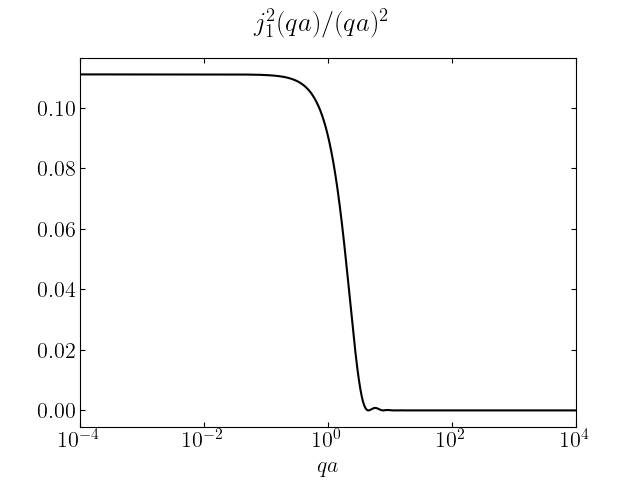
\includegraphics[width=0.8\textwidth]{p1.png} 
\end{center}
This indicates a sharp peak for $qa\lesssim1$. Thus, we can write $qa\approx
ka\theta$ and integrate for the total cross section
\begin{align}
    \sigma
    &=\pi k^4a^6\abs{\epsilon_r-1}^2\int_{-1}^1d(\cos\theta)
    \frac{j_1^2(ka\theta)}{(ka\theta)^2}\qty(1+\cos^2\theta)\notag\\
    &\approx\pi k^4a^6\abs{\epsilon_r-1}^2\int_0^\infty\theta d\theta
    \frac{j_1^2(ka\theta)}{(ka\theta)^2}(1+\cos^2\theta)\notag\\
    &=\pi k^2a^4\abs{\epsilon_r-1}^2\int_0^\infty
    xdx\frac{j_1^2(x)}{x^2}\qty[1+\cos^2\qty(\frac{x}{ka})]\notag\\
    &\approx 2\pi k^2a^4\abs{\epsilon_r-1}^2\int_0^\infty
    dx\frac{j_1^2(x)}{x}\notag\\
    &\approx\frac{\pi}{2}k^2a^4\abs{\epsilon_r-1}^2
\end{align}
where we have let $x/ka\to0$ since $ka\gg 1$ and numerically integrated the
integral in the final equality to be approximately $\pi/4$.
\end{solution}
\end{problem}
\newpage
%%%%%%%%%%%%%%%%%%%%%%%%%%%%%%%%%%%%%%%%%%%%%%%%%%%%%%%%%%%%%%%%%%%%%%%%%%%%%%%    
\end{document}
